% !TEX root = ../Thesis.tex
\chapter{Introduction}

Sudoku puzzles excite, as the rather simple task of filling out a grid with numbers becomes a demanding challenge just by stating a small set of rules that must be followed. For a $9 \times 9$ grid of cells which may already contain numbers, the original Sudoku rules every puzzle solver must follow are: A number with a value from 1 to 9 must be placed in each cell, and every number may appear only once per column, row and marked $3\times3$ box. An example of a normal Sudoku Puzzle and its solution is shown in Figures \ref{fig:SudokuManOfMystery} and \ref{fig:SudokuManOfMysterySolution}.

\begin{figure}
\vspace{2.5mm}
\centering
\begin{minipage}{.4\textwidth}
    \centering
    \captionsetup{justification=centering,margin=0cm}
    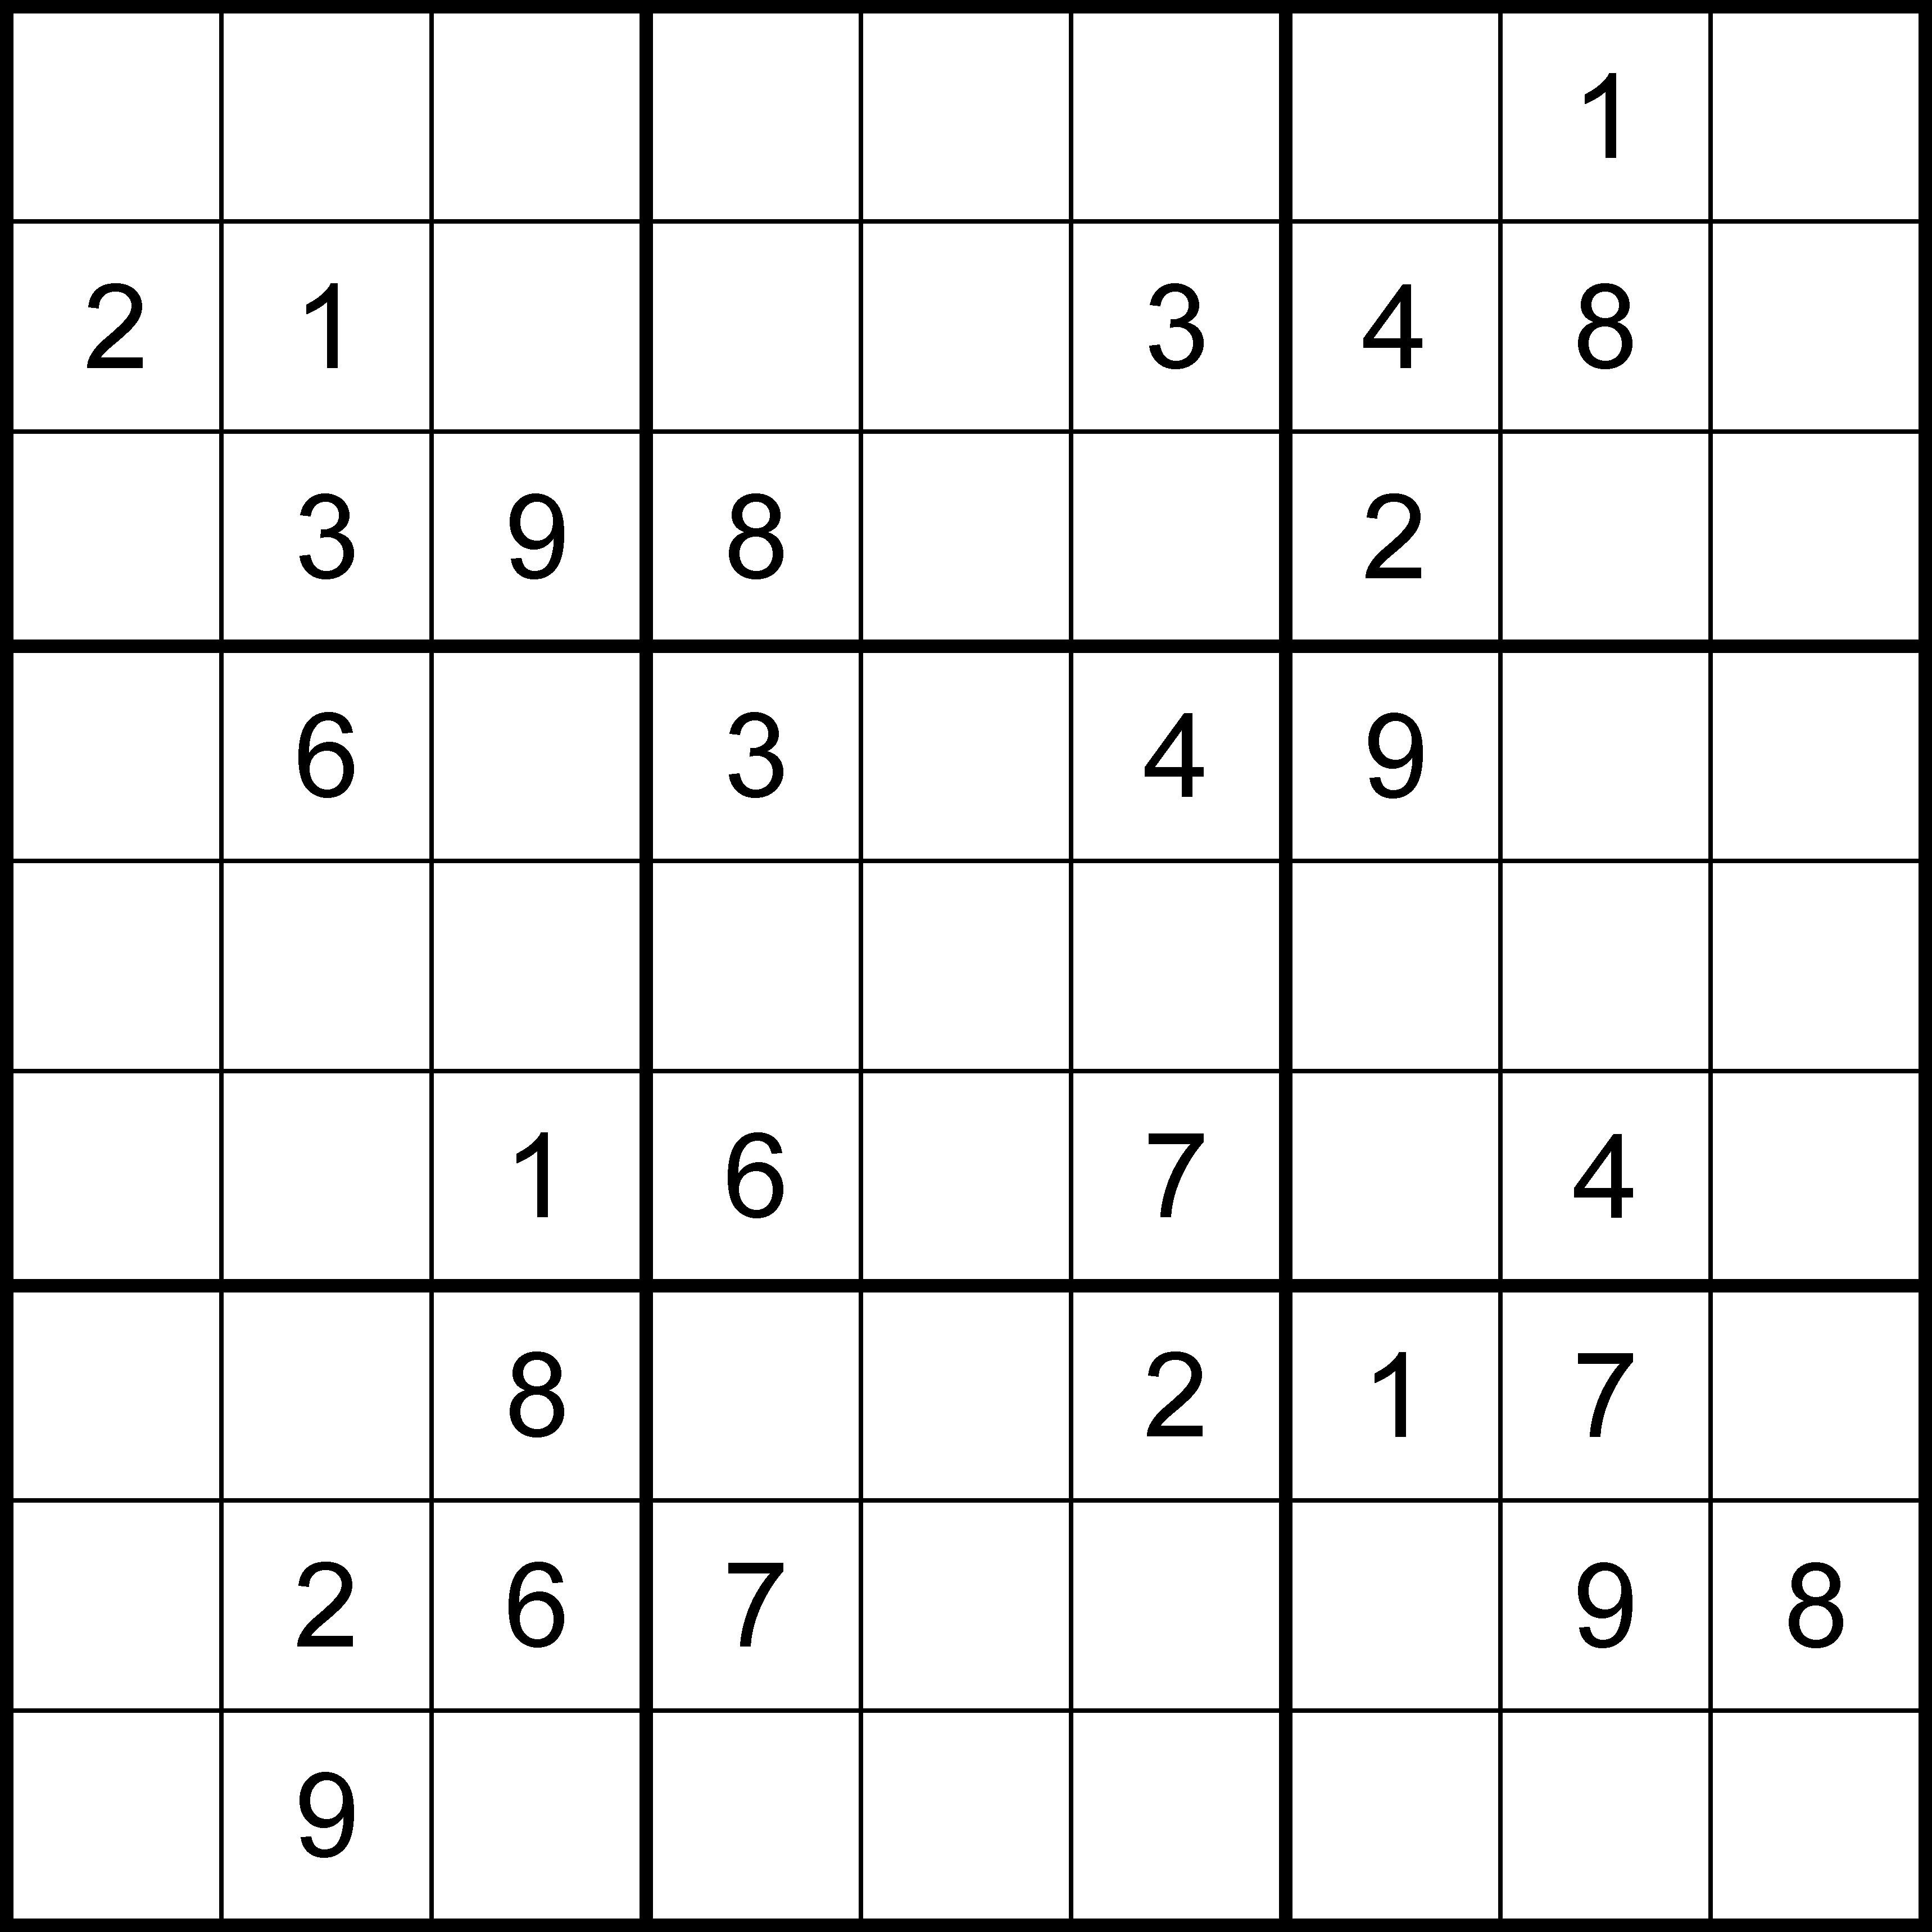
\includegraphics[width=.8\textwidth]{Figures/SudokuManOfMystery.png}
    \captionof{figure}{Normal Sudoku Puzzle,\\CTCGH \cite{CrackingTheCryptic2021} page 42}
    \label{fig:SudokuManOfMystery}
\end{minipage}%
\begin{minipage}{.4\textwidth}
  \centering
    \captionsetup{justification=centering,margin=0cm}
    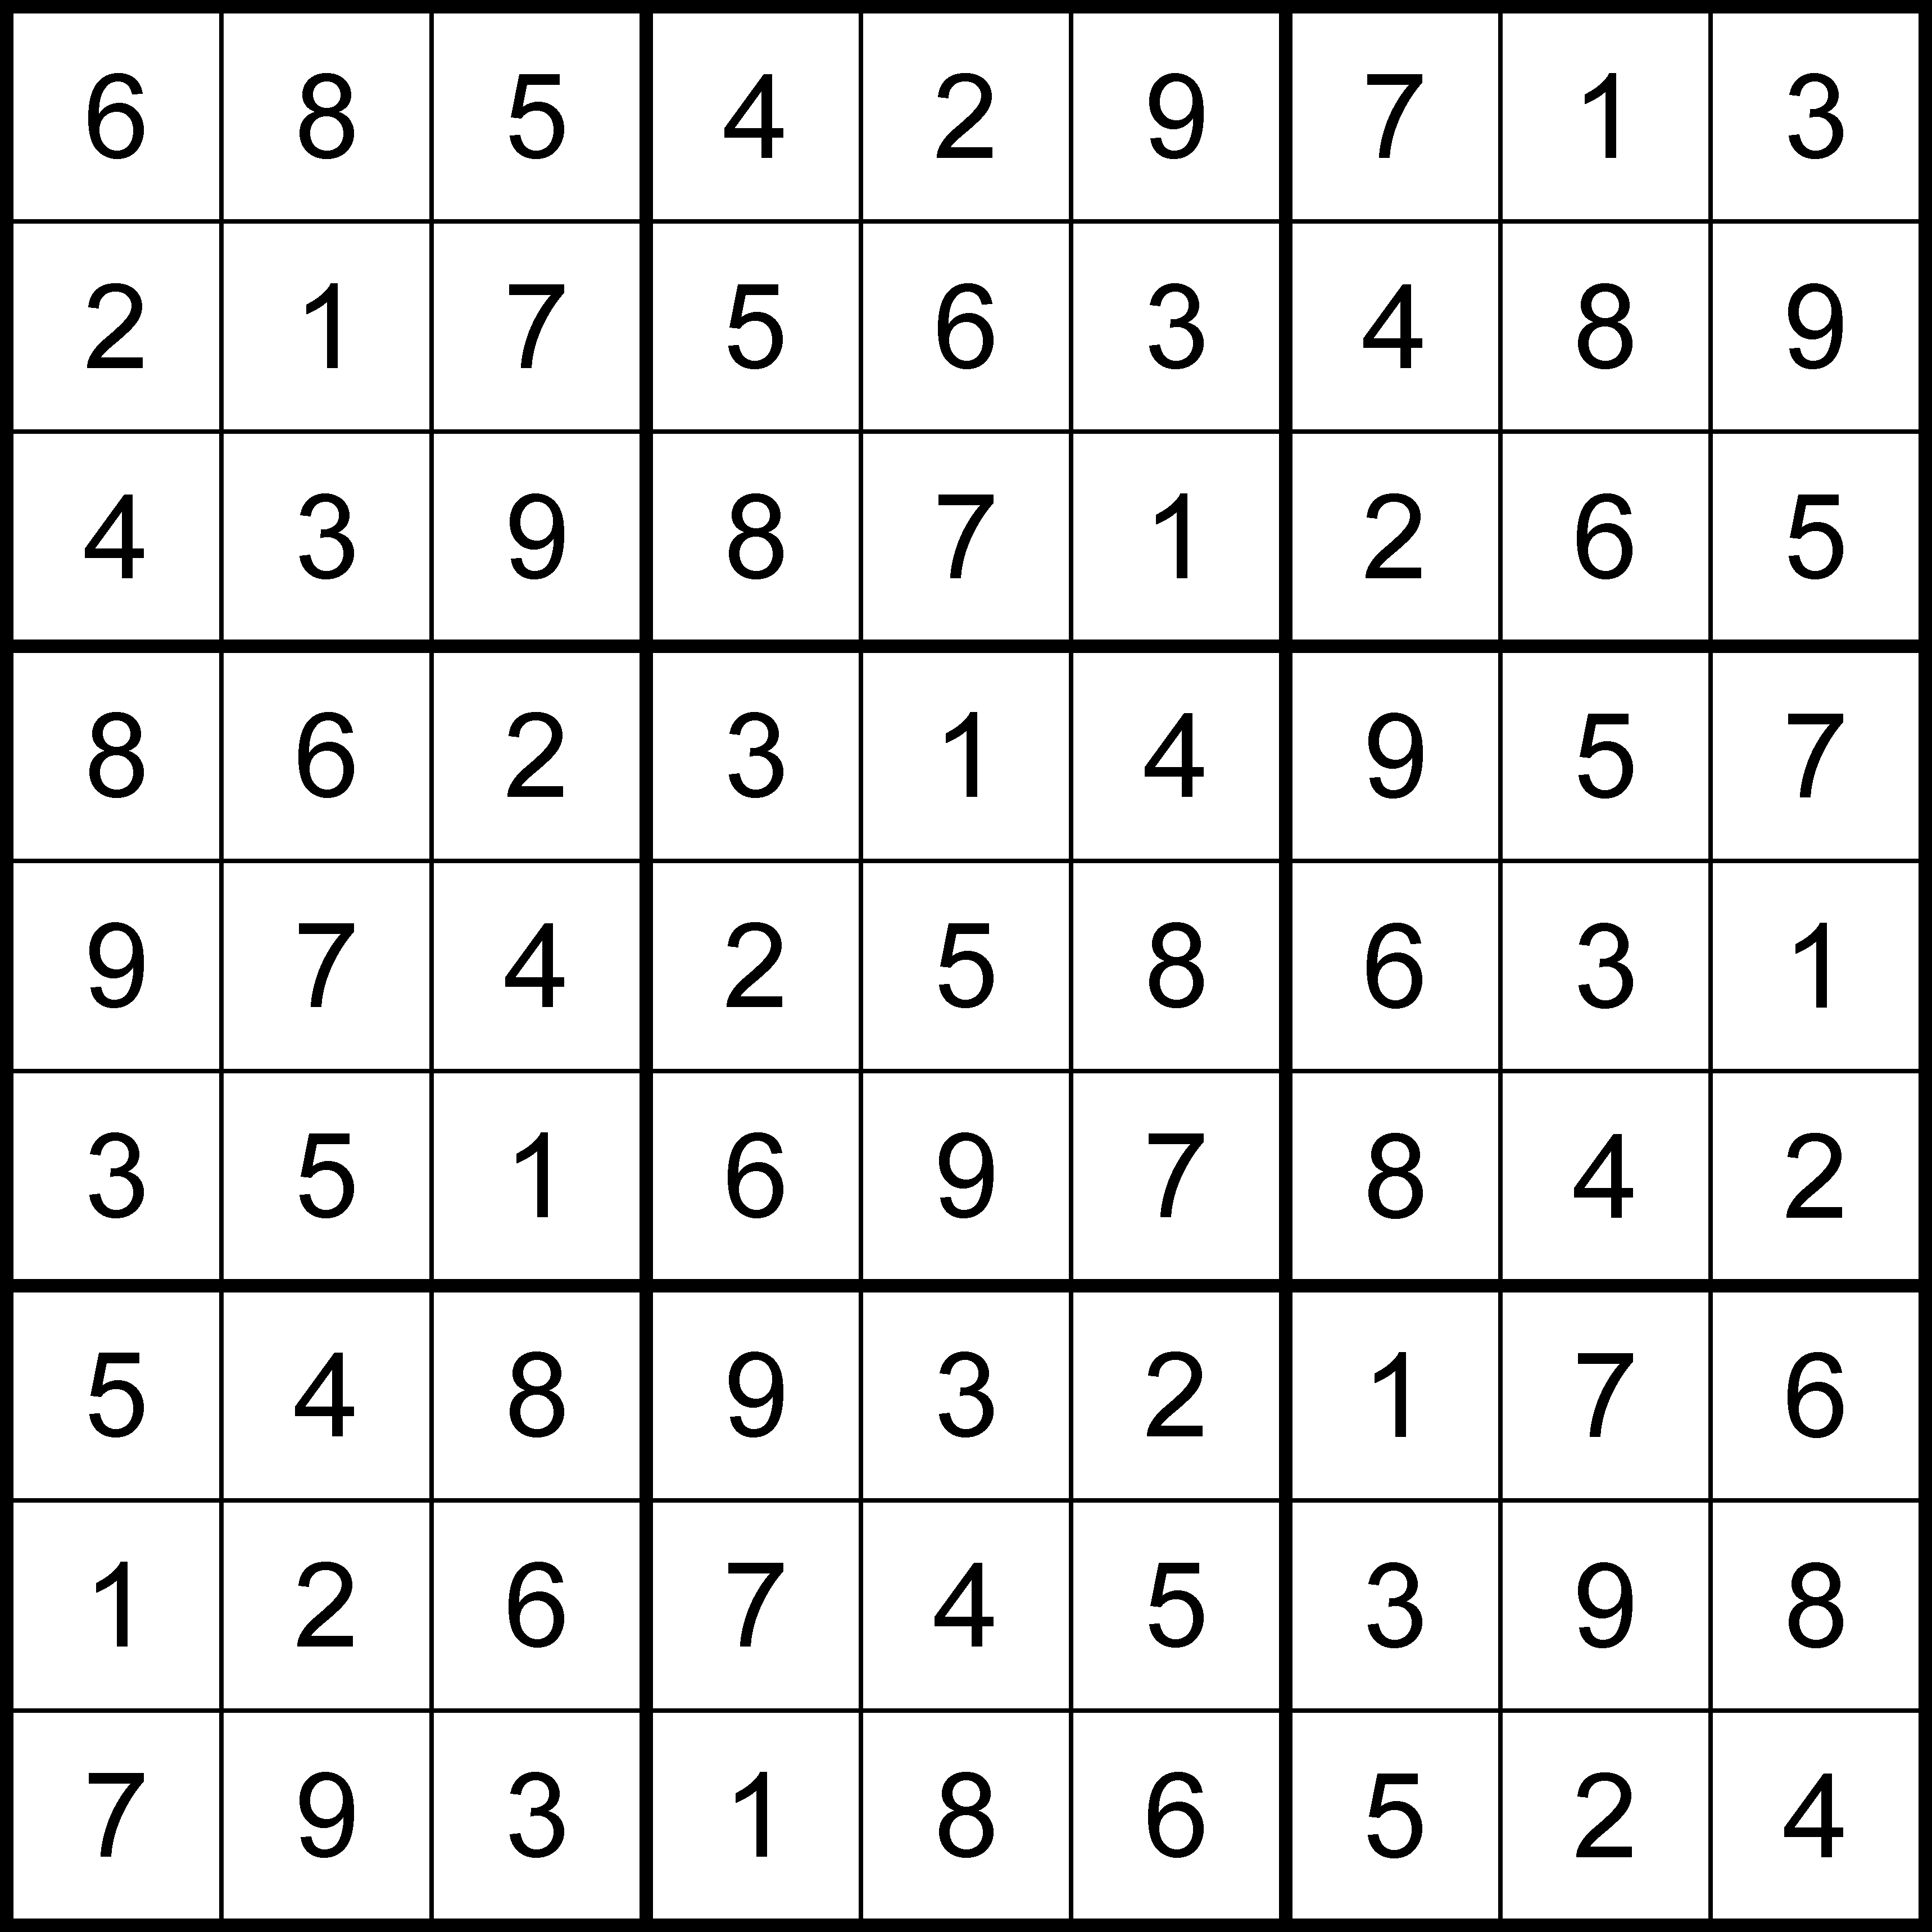
\includegraphics[width=.8\textwidth]{Figures/SudokuManOfMysterySolution.png}
    \captionof{figure}{Solution to Puzzle\\in Figure \ref{fig:SudokuManOfMystery}}
    \label{fig:SudokuManOfMysterySolution}
\end{minipage}
\end{figure}

Using these rules, the puzzle in its original form was first seen in the early 80s and established itself as one of the most popular logic puzzles in the last few decades. Since the mid-2000s, Sudokus also became an inherent part of the puzzle section in many newspapers and gained a fan community of puzzlers eager to develop and solve more challenging riddles. Around this time, researchers also started publishing first papers analysing Sudokus. For example, in 2006, it was shown by \cite{Felgenhauer2006MathematicsOS} that there are $6.671\times 10^{21}$ valid $9\times 9$ Sudoku grids. In the same year, Lynce and Ouaknine published a paper \cite{Lynce2006SudokuAsASATProblem} showing how Sudoku Puzzles can be encoded into logical formulas in a way that SAT-solvers can be used to find their solutions. SAT-solvers are suitable for solving Sudokus because most of the puzzles are “well-formed”, which means they only have one solution that is deducible without ambitions. Or, as \cite{Lynce2006SudokuAsASATProblem} states, ``Such puzzles are meant to be solved without search, i.e., merely with reasoning.''\\
\\
In this thesis, we aim to go one step further and find encoding methods for Sudoku Variants that are based on original Sudoku but augment the rules with additional requirements that solutions must fulfil. Our source of choice for such rather unconventional Sudoku Variants and rules will be the book ``Cracking The Cryptic Greatest Hits'' (\emph{CTCGH}) \cite{CrackingTheCryptic2021}, which presents a collection of the most unique, entertaining but also demanding Sudoku Variants the puzzle community came up with until today. The book was published after a successful Kickstarter campaign by Mark Goodliffe and Simon Anthon, which run one of the most famous Youtube channels focused on Sudokus: ``Cracking The Cryptic''\cite{ChannelCrackingTheCryptic}. In their videos, they present and solve puzzles sent to them from people all around the world, allowing them to create this phenomenal assortment of diverse Sudoku Variants.\\
\\
To get a foretaste of the variants we will work with, one may solve the Sudoku depicted in Figure \ref{fig:Thermo2020}. The normal Sudoku rules apply, but instead of already filled out cells, seven so-called \emph{Thermometers} are placed on the grid. For each Thermometer, it must hold that starting from the bulb, the cell values along the Thermometer can only strictly increase. As one will see, this already suffices to guarantee the uniqueness of the solution.\\
\\
As we intend to make the encodings of different rules compatible with each other, it will be possible to encode and solve new Sudoku Variants formed by arbitrarily combining said rules. To test our encodings, though, we will use puzzle instances from CTCGH and state of the art SAT-solvers like MiniSat. Comparing the encodings and the performance of the SAT-solvers working on them, we will show that for most puzzle instances from CTCGH, SAT-solvers can find a solution within seconds. However, we will also find exceptions to this, with Sudoku Variants that require extensive encodings and comparably high solving times by the SAT-solvers, revealing that the task of encoding and solving these special Sudoku Variants is by no means a trivial one.\\
\\
Because we will examine many Sudoku Variants with rules involving sums, we also want to further elaborate on the encoding of Pseudo Boolean Constraints. Following the ideas of \cite{Een2006TranslatingPC}, we will show how Binary Decision Diagrams and Adder Networks can be used to encode Pseudo Boolean Constraints and how the two methods compare to each other.

\begin{figure}
\centering
\captionsetup{justification=centering,margin=0cm}
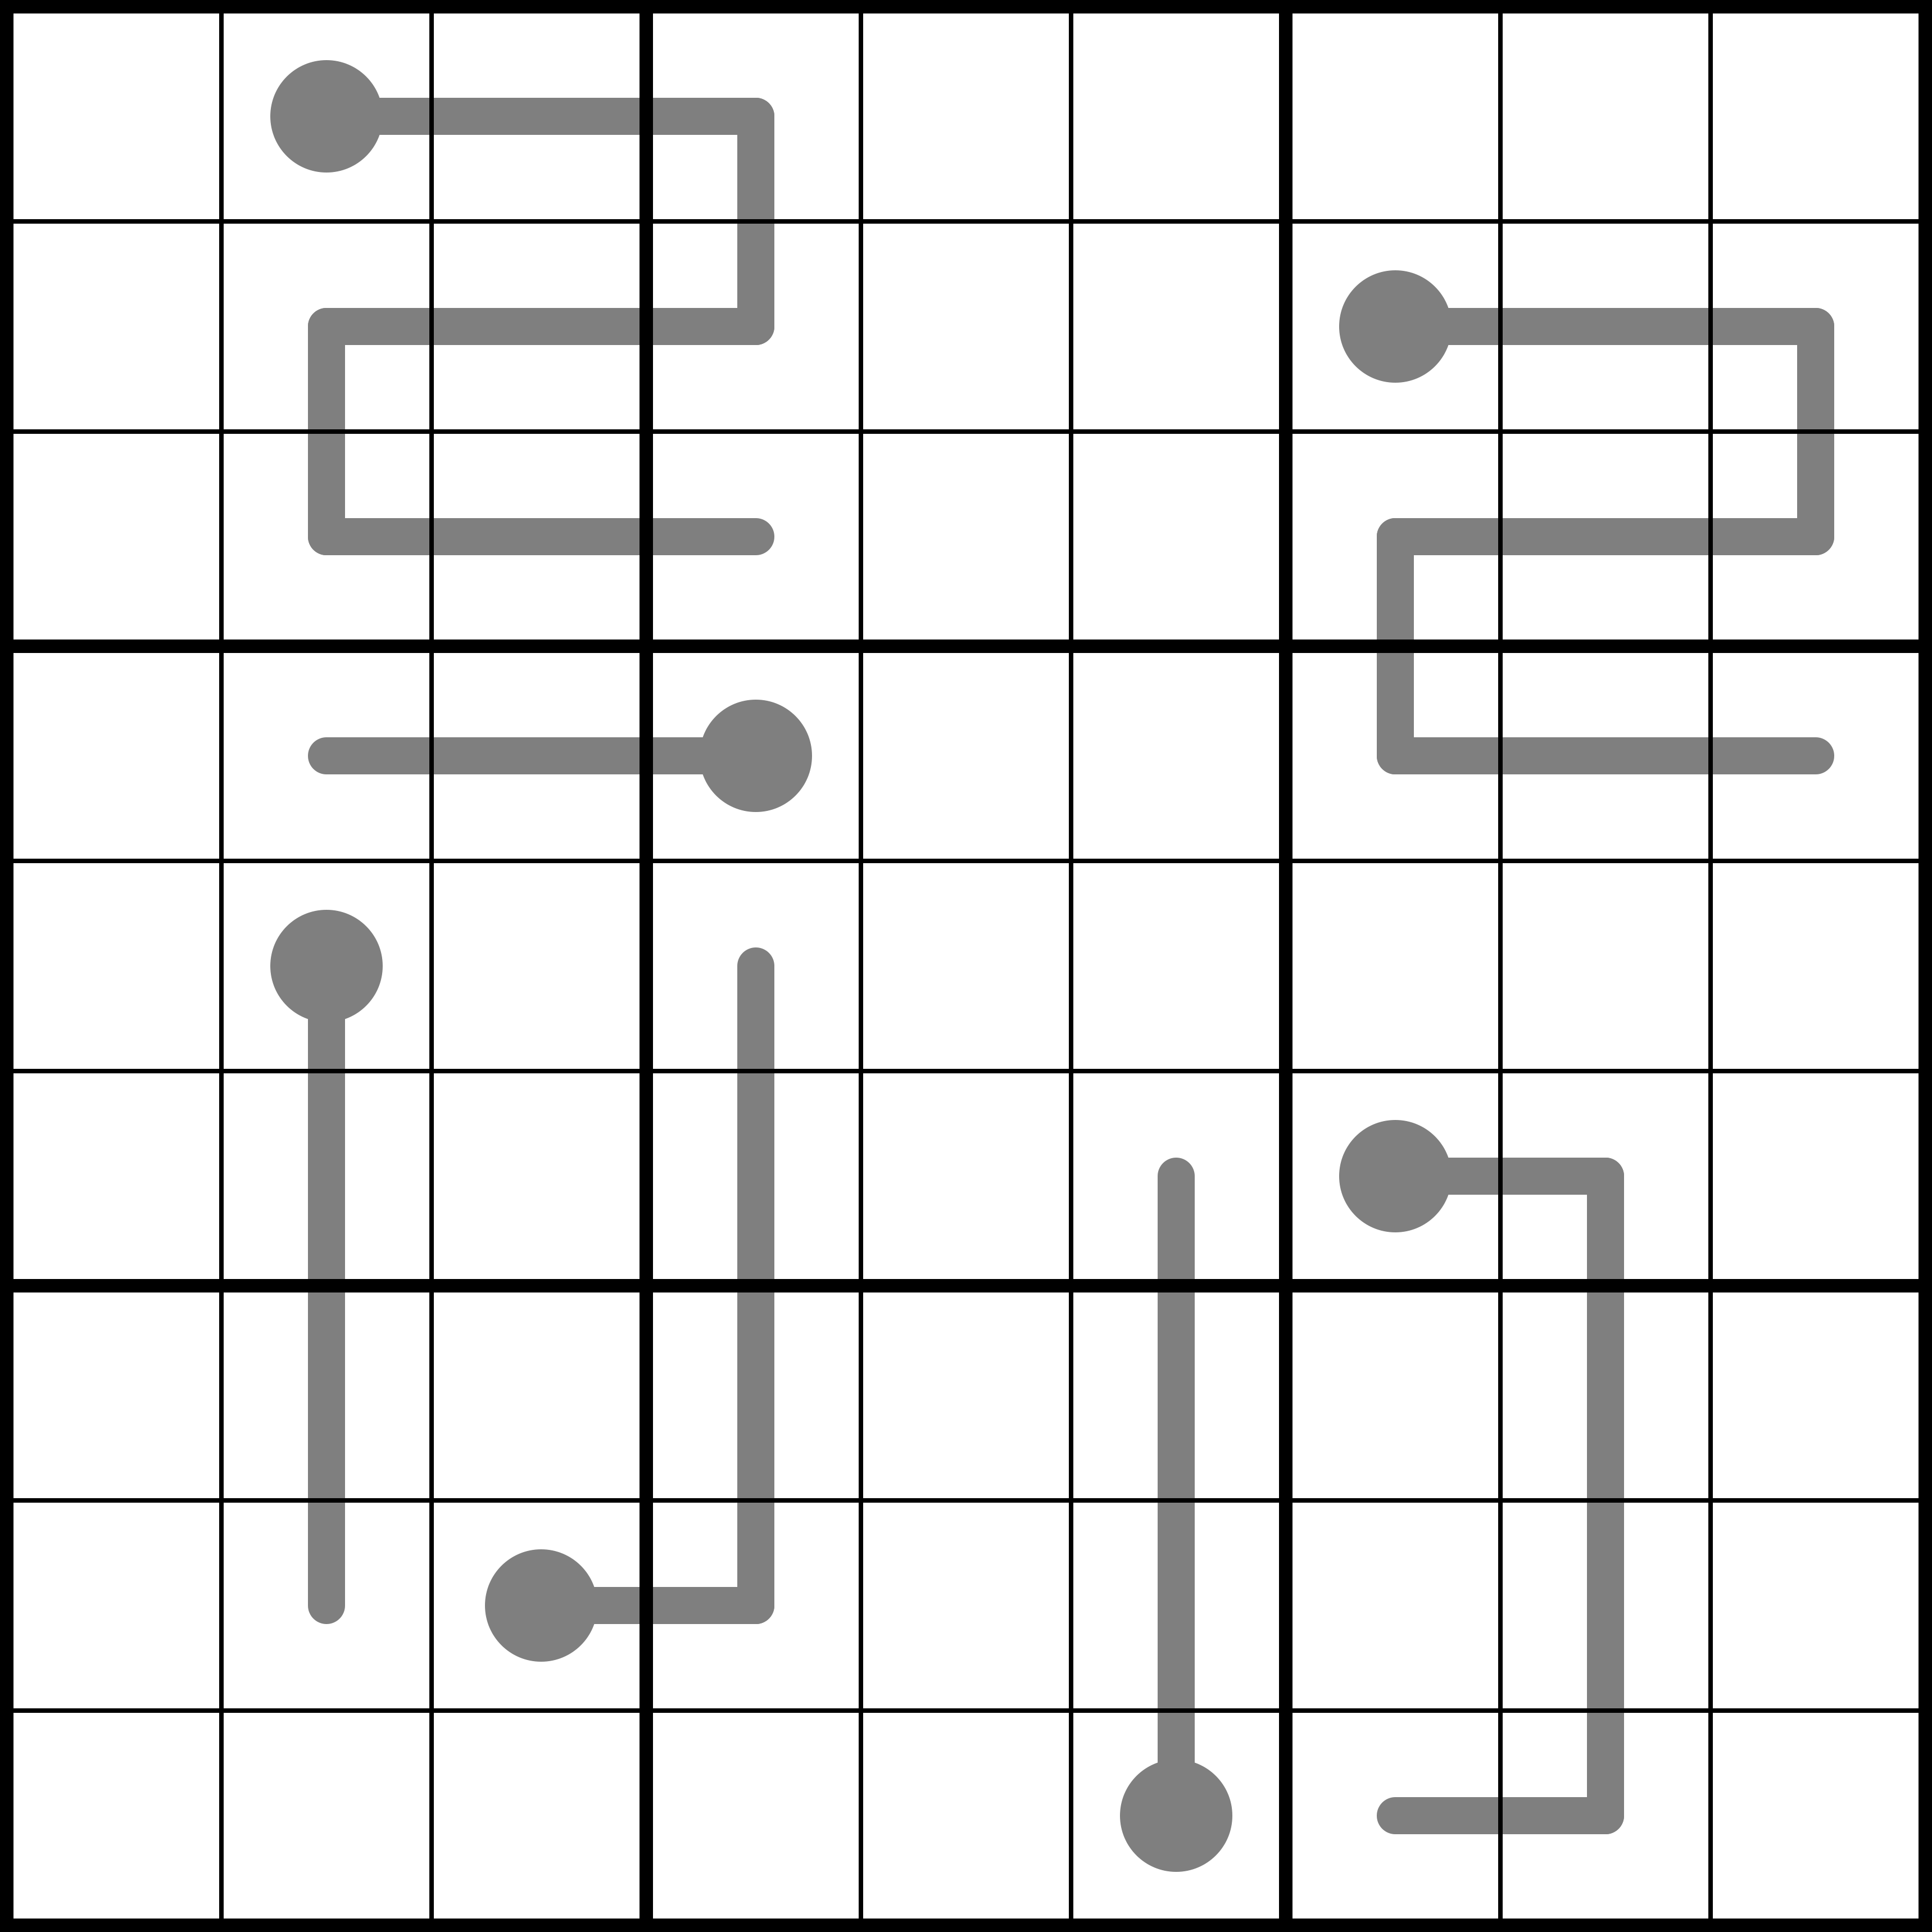
\includegraphics[width=\textwidth]{Figures/Thermo2020.png}
\caption{Example of a Sudoku Puzzle using Thermometers,\\puzzle by Akash Doulani, CTCGH page 15 \cite{CrackingTheCryptic2021},\\this is a corrected version, available at \cite{OnlineSolutionThermo2020} }
\label{fig:Thermo2020}
\end{figure}





